%
% Copyright (C) 2017 Jan Nowotsch
% Author Jan Nowotsch	<jan.nowotsch@gmail.com>
%
% Released under the terms of the GNU GPL v2.0
%



\section{Atmel \avr}
	This section summarises some critical specifics of the \avr architecture.

	\subsection{Linker sections}
		The \avr memory is split into code (flash) and data (\gls{sram}). Since the \gls{sram} is volatile memory all data that belongs to linker sections such as .data and .bss are initially programmed to the flash memory and need to be copied to \gls{sram} during startup. The respective section offsets are defined in the linker scripts used to link the kernel (\fileref{scripts/linker/kernel\_avr.lds}). In case of the .data section, the base address within the flash is defined as \lstinline{__data_load_start} while the end address is defined as \lstinline{__data_load_end}. The respective target address in \gls{sram} are defined in \lstinline{__data_start} and \lstinline{__data_end}.

		The memory layout is defined through the device tree. As described above .data and .bss sections are programmed to flash and loaded to \gls{sram} at runtime. Hence, the respective sections of kernel and init application require a share of the flash memory as well as the \gls{sram}. The required space in the flash memory has to be respected such, that the size has to be large enough to hold the kernel .text, .data and .bss sections. The required space in \gls{sram} needs to be considered when defining the kernel memory layout through, i.e. kernel image, stack and heap, as well as process heap and init ram file system. An exemplary memory layout is shown in Figure~\ref{fig:avr_memory_layout}.
		\begin{figure}[h]
			\centering	
			\includegraphics[scale=.75]{arch/avr_memory_layout}
			\caption{Exemplary \avr memory layout.}
			\label{fig:avr_memory_layout}
		\end{figure}

	\subsection{Interrupt Handling and Reset}
		At reset execution is started at the processor reset address. The location of the reset address is controlled through the \lstinline{BOOTRST} fuse and might be at the start of the application section (\lstinline{0x0}) or the boot loader. The start of the boot loader section is further controlled through the \lstinline{BOOTSZ0, BOOTSZ1} fuse bits. Depending on the memory configuration of the target controller the boot loader start address may vary.
		
		Depending on the fuse bit configuration the kernel base address has to be set through the \lstinline{kernel_flash} memory node in the device tree. \remark{It shall be noted that the application flash is address is 2-byte chucks, hence addresses listed in the manual need to be multiplied by two in order to get the byte address.}

		The location of the interrupt vectors (except the reset vector) is controlled through \lstinline{MCUCR[IVSEL]}. They can either be placed at the start of the application section or the boot loader section. In the current implementation all interrupt vectors, including the reset vector, are mapped to the same location depending on the \lstinline{kernel_flash} memory node in the device tree.

	\subsection{Program Memory Specifics of \atmega controllers}
		\subsubsection{Word vs. Byte Addressing}
			The \avr program memory is addressed in 2 byte chunks, hence if an address needs to be set or read, it needs to be converted properly. For instance, if the return address of an interrupt shall be printed, the address needs to be multiplied by 2. Likewise, if a byte address shall be set, as thread entry point for instance, it needs to be divided by 2.

		\subsubsection{Return Addresses}
			Return addresses for calls and interrupts are stored on the stack using big endian even though the \atmega architecture as such uses the little endian format. That is, the high order 8 bits of the address are stored at lower address, while the low order 8 bits are stored at higher address, cf. \ref{fig:atmega_return_address} as an example.
			\begin{figure}[h]
				\centering	
				\includegraphics[scale=.75]{arch/atmega_return_address}
				\caption{Example how to place the return address 0x9000 in memory.}
				\label{fig:atmega_return_address}
			\end{figure}
